\newpage
\section{Differentiable Appearance Acquisition}
可微分采集材质?

\subsection{Introduction}

渲染材质需要知道颜色, 反射率, 反射类型(漫, 全), 反射函数(输入观察角度, 输出颜色)

Light/material interaction: 吸收, 反射, 穿透

\begin{figure}[!htb]
    \centering
    \includegraphics[width=0.42\textwidth]{pic/ACG4/光}
    \caption{Light/material interaction}
\end{figure}

要数字化光的特性. 

\subsection{Reflection Models}
\subsubsection{BRDF}
Bidirectional Reflection Distribution Function(双向反射率分布函数) $f(i,o)$, 四维函数(只要方向)

若固定 $i$(入射), 函数退化为描述出射光的分布. 
\begin{figure}[!htb]
    \centering
    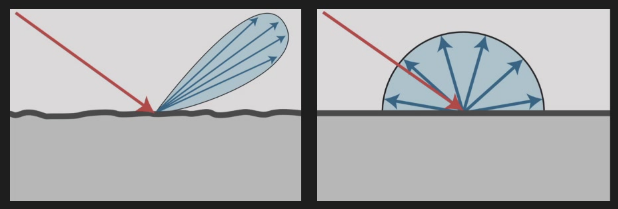
\includegraphics[width=0.309\textwidth]{pic/ACG4/BRDFfi.png}
    \caption{BRDF fixing $i$}
\end{figure}


\subsubsection{Perfect Mirror Reflection}
完美镜面反射
\begin{figure}[!htb]
    \centering
    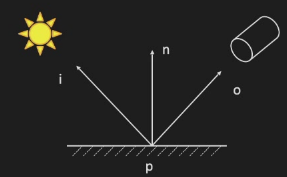
\includegraphics[width=0.309\textwidth]{pic/ACG4/Perfect Mirror Reflection}
    \caption{Perfect Mirror Reflection}
\end{figure}
光的方向相反是为了计算少一个负号, 方便, 算是某种约定. 

计算出射光方向, 再比较是否一致.
\begin{align*}
    -r=-(i-\braket{i,n}n)+\braket{i,n}n=2\braket{i,n}n-i
\end{align*}
\begin{figure}[!htb]
    \centering
    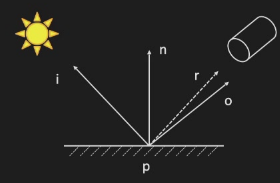
\includegraphics[width=0.309\textwidth]{pic/ACG4/计算}
    \caption{naive}
\end{figure}


计算半向量(Half Vector),
\begin{align*}
    h=\frac{i+o}{\norm{i+o}}
\end{align*}
判断其是否与 $n$ 共线. 
\begin{figure}[!htb]
    \centering
    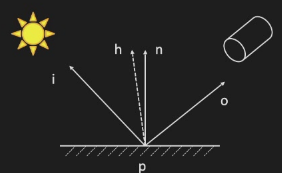
\includegraphics[width=0.309\textwidth]{pic/ACG4/Half Vector}
    \caption{Half Vector}
\end{figure}

\paragraph{Fresnel Reflection Term}
反射依赖于观察角度. 

解麦克斯韦方程组求反射率, 也可以用逼近

\paragraph{Schilick's Approximation}
\begin{align*}
    R(\theta)&=R_0+(1-R_0)(1-\cos\theta)^5\\
    R_0&=\left( \frac{n_1-n_2}{n_1+n_2} \right)^2
\end{align*}


\subsection{Microfacet-Based Models}
所有真实世界的材料都可以由小镜子建模而成. 通过控制小镜子(microfacet)法向量的朝向控制材质反射.

\begin{align*}
    f(i,o)=\frac{F(i,h)G(i,o,h)D(h)}{4(n,i)(n,o)}
\end{align*}

\begin{itemize}
    \item $F(i,h)$ Fresnel Reflection Term
    \item $D(h)$ 小镜子法向量分布函数, 发生$n=h$镜面反射的小镜子的概率. 
    \item $G(i,o,h)$ 考虑小镜子之间的遮挡(Shadowing and Masking).
    \begin{figure}[!htb]
        \centering
        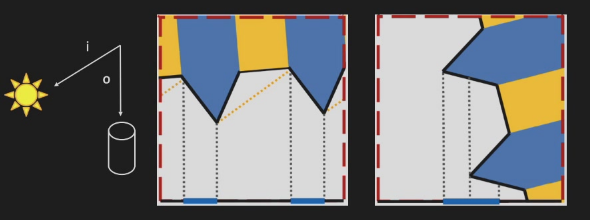
\includegraphics[width=0.42\textwidth]{pic/ACG4/Shadowing and Masking}
        \caption{Shadowing and Masking}
    \end{figure}
    \item 分母是依据视角的衰减项
\end{itemize}

\subsubsection{Example: Cook-Torrance Model}
\begin{align*}
    D&= \frac{e^{\frac{-\tan^2(\alpha)}{m^2}}}{\pi m^2\cos^4 (\alpha)}, \alpha = \arccos(n\cdot h)\\
    G&= \min\left( 1, \frac{2(h\cdot n)(o\cdot n)}{o\cdot h}, \frac{2(h\cdot n)(i\cdot n)}{o\cdot h} \right)
\end{align*}

仅需要一个 $m$ 参数即可控制高光.

\subsection{Anisotropic BRDF}
各向异性的高光. 因为小尺度上材质的方向性.

\subsection{Diffuse Reflection}
漫反射. 光在各个方向上反射相同. 

Lambertian model
\begin{align*}
    f(i,o)=constant
\end{align*}
这里仅仅是为了描述方便, 物理上难以实现. 

\begin{align*}
    f(i,o)(i,n)=\left[ \frac{\rho_d}{\pi}+\rho_s\cdot f_{spec}(i,o) \right](i,n)
\end{align*}
$\rho_d, \rho_s$ 是 diffuse/specular coefficient

\subsection{Measured Data}
使用函数列表存储. 优点:真实, 缺点:开销大.


\href{http://www.disneyanimation.com/technology/brdf.html}{BRDF Explorer}


\subsection{Differentiable Acquisition of Visual Information}
end-to-end(端到端) 

深度学习的端到端需要物理信息到最后的结果. 软硬件一起考虑. 所以说是可微分的数据获取(Differentiable Acquisition), 可以通过梯度优化. 

数据的信息量很多, 想少采集必须使用强先验补足信息. 

用神经网络的参数控制现实世界.(这里是控制灯的亮度) 具体来说就是优化参数, 也等价于优化控制. 

用已有数学模型生成训练数据. 

\subsubsection{Efficient Reflectance Capture Using an Autoencoder}
一作是本科生, 应该大三才开始做的, 这篇文章拿到了一个很好的奖, 听下来确实非常精妙, 很有收获.


文章的目的是为了快速重建材质的 BRDF 函数. 

\begin{figure}[!htb]
    \centering
    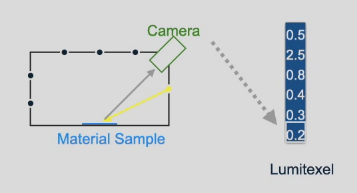
\includegraphics[width=0.309\textwidth]{pic/ACG4/device}
    \caption{device}
\end{figure}

Lumitexel 是一个像素点, 每个灯的角度获得的 BRDF 输出的集合, 包含了最多的信息. 


\paragraph{naive 方法} 就是使用打表的方法记录现实的 BRDF, 即记录每个像素的 Lumitexel. 开启一个灯珠, 拍一张照, 获得 BRDF 的一个角度的输出, 换一个灯珠如此重复, 直到获得所有灯珠角度的输出, 就算记录了 BRDF 函数. 

缺点: 开销大, 时间长. 灯珠有近 10000 个.

\paragraph{论文方法} 以某种方式组合灯珠, 获得一些观测值(32 个左右), 再通过这些值重建出原本的 Lumitexel. 组合方式与重建方式通过神经网络训练而来.

\begin{figure}[!htb]
    \centering
    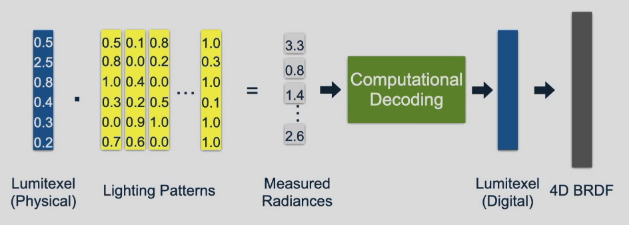
\includegraphics[width=0.42\textwidth]{pic/ACG4/pipline.png}
    \caption{Pipeline}
\end{figure}

原理是灯亮度与那个像素 Lumitexel 的点积就是观测值, 这样求 Lumitexel 就相当于解线性方程组, 但是妙就妙在方程组的系数是通过学习而来的. 他用第一层参数控制了灯组合方式. 这样训练时就可以调整组合, 获得更好的数据. 

\begin{figure}[!htb]
    \centering
    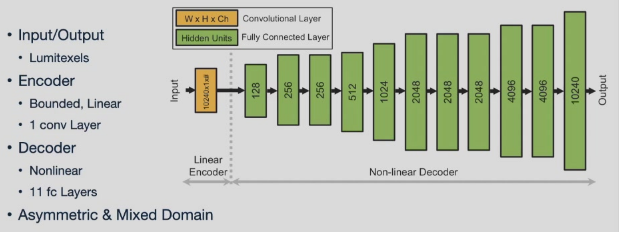
\includegraphics[width=0.42\textwidth]{pic/ACG4/L-DAE.png}
    \caption{L-DAE}
\end{figure}

训练数据的来源于成熟的 BRDF 函数估计与拟合公式, 从经典材质上训练的网络参数可以去采集其他材质, 做到很好的重建. 